\normalfalse \difficiletrue \tdifficilefalse
\correctionfalse

%\UPSTIidClasse{11} % 11 sup, 12 spé
%\newcommand{\UPSTIidClasse}{12}

\exer{EPAS$\star$ \label{C2:09:64}}

\setcounter{question}{0}\UPSTIcompetence[2]{C2-09}
\index{Compétence C2-09}
\index{TEC}
\index{Théorème de l'énergie cinétique}
\index{EPAS}
\ifcorrection
\else
\marginnote{\textbf{Pas de corrigé pour cet exercice.}}
\fi

\ifprof
\else
On suppose que le système de commande du déploiement permet d’obtenir une vitesse de la plateforme
trapézoïdale :
\begin{itemize}
\item une première phase de mouvement uniformément accéléré, d’accélération $\Gamma_0$;
\item une deuxième phase de mouvement uniforme, de vitesse $V_0$;
\item une dernière phase de mouvement uniformément décéléré, d’accélération $-\Gamma_0$.
\end{itemize}
 
\begin{figure}[H]
\centering
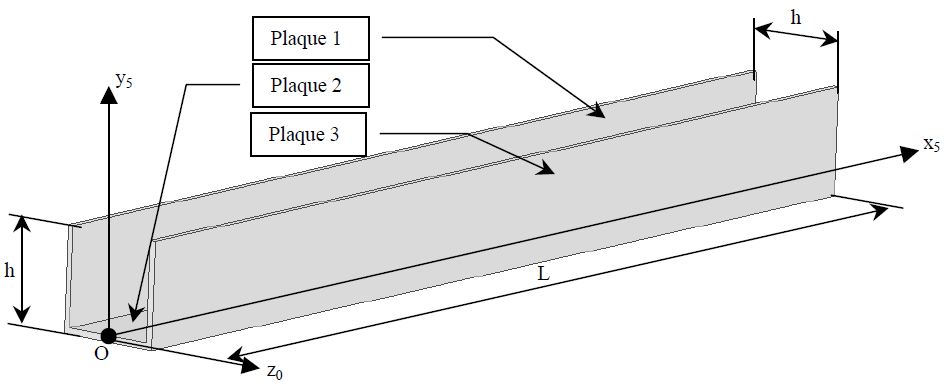
\includegraphics[width=\linewidth]{64_01}
%\caption{Représentation en coupe du banc BALAFRE \label{fig_50_01}}
\end{figure}


On note $\rep{0}=\repere{O}{x_0}{y_0}{z_0}$ le repère lié au châssis et
$\rep{1}=\repere{O}{x_1}{y_1}{z_0}$ le repère lié au berceau.

\textbf{Le parc échelle :} le parc échelle est redressé d’un angle $\theta$ constant par rapport à l’horizontale.
Les plans du parc échelle ont tous la même masse notée $M$. Leur centre de gravité sera noté $G_i$,
$i$ étant le numéro du plan.

Chaque plan du parc échelle se translate par rapport au châssis, suivant $\vx{1}$ à une vitesse deux
fois plus grande que le plan suivant :  $\vectv{P}{\text{Plan}_i}{\rep{0}}=2\vectv{P}{\text{Plan}_{i+1}}{\rep{0}}$

Le guidage des plans les uns par rapport aux autres engendre des efforts s’opposants aux
mouvements que l’on modélisera par un glisseur dont le module de la résultante sera noté $F$
constant.

\textbf{La plate-forme :} la plate-forme de centre de gravité $G_P$ a une masse notée $m$, et se translate par rapport au
châssis suivant $\vx{1}$ à une vitesse notée $V(t)$.

\textbf{Le treuil :} un treuil de rayon $R$, tournant à une vitesse de rotation notée $\omega$, entraîne le câble principal
dont les extrémités sont fixées au plan n°3. Le moment d’inertie du treuil par rapport à son axe de rotation, sera noté $I$.
Le moment du couple moteur exercé par l’ensemble moto réducteur hydraulique sera noté $C$.

\begin{figure}[H]
\centering
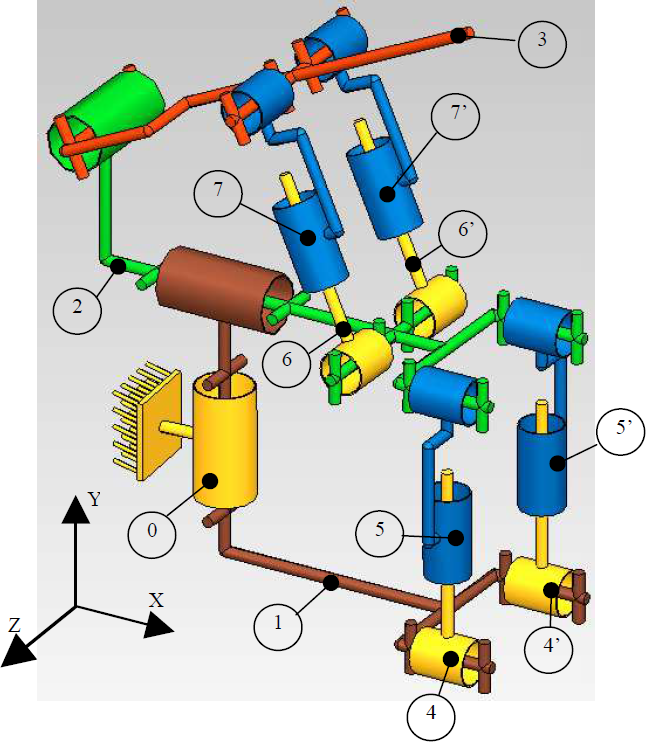
\includegraphics[width=\linewidth]{64_02}
%\caption{Représentation en coupe du banc BALAFRE \label{fig_50_01}}
\end{figure}
\fi


\question{Déterminer l’énergie cinétique galiléenne de la plate-forme et des quatre plans
du parc échelle en fonction de $V(t)$ et des différentes masses.}
\ifprof
\else
\fi

\question{Déterminer l’énergie cinétique galiléenne du treuil en fonction de $V(t)$.}
\ifprof
\else
\fi

\question{Déterminer la puissance des actions extérieures à l’ensemble \{treuil+parc échelle+plate-forme\} en fonction de $V(t)$.}
\ifprof
\else
\fi

\question{Déterminer la puissance des actions intérieures de ce même ensemble en fonction de $V(t)$.}
\ifprof
\else
\fi

\question{En déduire le moment du couple moteur nécessaire pendant la première phase
de mouvement.}
\ifprof
\else
\fi



\ifprof
\else
\footnotesize
\begin{itemize}
\item $\ec{E}{0}=\dfrac{1}{2}\left(m+\dfrac{21}{16}M \right)V^2$.
\item $\ec{CT}{0}=\dfrac{1}{2}\dfrac{I}{16R^2}V^2$.
\item $P_{\text{ext}}=V\left(\dfrac{C}{4R}-g\left(m+\dfrac{7}{4}M \right)\sin\theta\right)$.
\item $P_{\text{int}}=-FV$.
\item $4R\left[\left(m+\dfrac{21}{16}M+\dfrac{I}{16R^2}\right)\Gamma_0 +F+g\left( m+\dfrac{7}{4}M\right)\sin \theta \right]$.
\end{itemize}
\normalsize
\begin{flushright}
\footnotesize{Corrigé  voir \ref{C2:09:64}.}
\end{flushright}%
\fi